
\section*{Handschriftherkenning}
\flushright
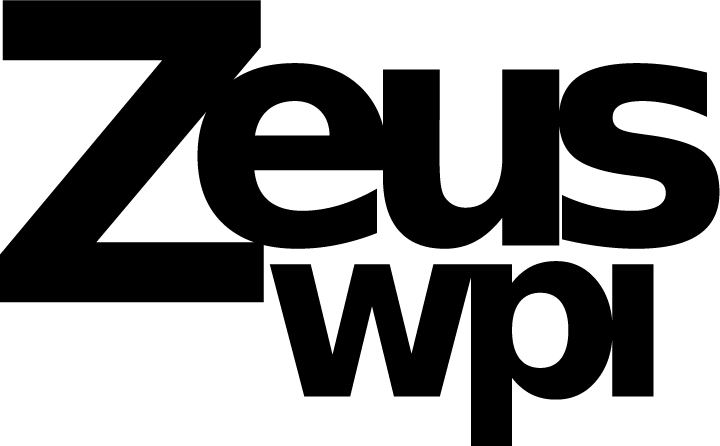
\includegraphics[width=4em]{logo-new.png}
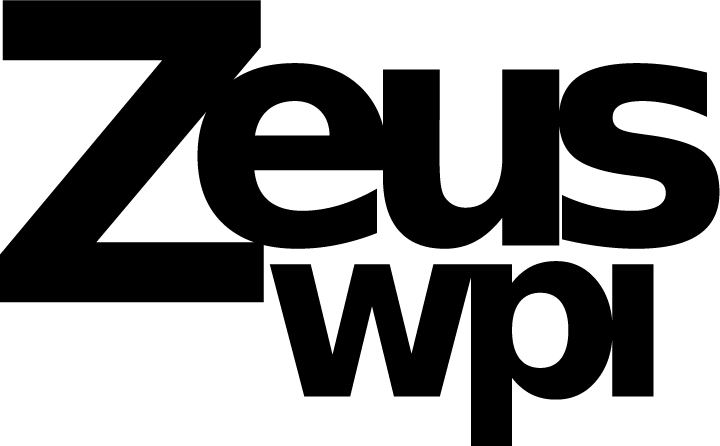
\includegraphics[width=4em]{logo-new.png}
\flushleft

Optical character recognition (OCR) is een techniek die kan gebruikt worden om
ingescande afbeeldingen van handgeschreven, getypte of afgedrukte tekst om te
zetten naar ASCII-tekst die leesbaar is voor een computer. Deze techniek wordt
vaak gebruikt om afgedrukte teksten te digitaliseren zodat men ze elektronisch
kan doorzoeken, compacter kan opslaan, online kan weergeven, of ze automatisch
kan laten vertalen of voorlezen door een computer. OCR vormt een
onderzoeksdomein binnen de patroonherkenning, artifici\"ele intelligentie en
computervisualisatie.

In deze opgave werken we met tekstbestanden, waarvan de regels een aantal
handgeschreven karakters voorstellen. Het handschrift staat telkens in een
lettertype dat voldoet aan volgende voorwaarden:

\begin{itemize}
    \item alle regels hebben dezelfde lengte (inclusief spaties);
    \item gelijke handgeschreven karakters worden steeds op dezelfde manier
        weergegeven;
    \item verschillende handgeschreven karakters worden nooit op dezelfde manier
        weergegeven;
    \item de voorstelling van een handgeschreven karakter bevat nooit lege
        kolommen;
    \item tussen twee opeenvolgende handgeschreven karakters staan \'e\'en of
        meer lege kolommen;
    \item voor het eerste en na het laatste handgeschreven karakter staan nul of
        meer lege kolommen.
\end{itemize}

Een lege kolom is een kolom van de regels met handgeschreven tekst die enkel
bestaat uit spaties. Hieronder wordt de inhoud weergegeven van een dergelijk
tekstbestand dat een handgeschreven versie van de letters ocrrococo bevat. Klik
hier om een grafische voorstelling van de segmentatie van dit tekstbestand te
bekijken. Hierbij worden de segmenten aangegeven met een donkergrijze
achtergrond, en worden de regels die niet opgenomen worden in de
stringvoorstelling van segmenten met een rode lijn doorstreept.

\begin{verbatim}
 ##   ### # ## # ##  ##   ###  ##   ###  ##
#  # #    ## # ## # #  # #    #  # #    #  #
#  # #    #    #    #  # #    #  # #    #  #
#  # #    #    #    #  # #    #  # #    #  #
#  # #    #    #    #  # #    #  # #    #  #
 ##   ### #    #     ##   ###  ##   ###  ##
\end{verbatim}

De opgave bestaat erin om de inhoud van het tekstbestand om te zetten naar de
corresponderende reeks ASCII karakters.

\subsection*{Input}

Als input krijg je eerst een lijn die het aantal gevallen aanduid. Per geval
krijg je vervolgens een lijn met twee woorden. Het eerste woord is het begin van
de handgeschreven tekst. Het volgende woord is een geheel getal dat het aantal
lijnen dat de handgeschreven tekst in beslag neemt. Hierop volgt deze
handgeschreven tekst.

Merk op dat het gegeven woord telkens alle letters die later kunnen voorkomen
zal bevatten. Het is als het ware een alfabet voor de rest van de tekst.

\subsubsection*{Voorbeeldinput}

\begin{verbatim}
2
ocr 6
 ##   ### # ## # ##  ##   ###  ##   ###  ##
#  # #    ## # ## # #  # #    #  # #    #  #
#  # #    #    #    #  # #    #  # #    #  #
#  # #    #    #    #  # #    #  # #    #  #
#  # #    #    #    #  # #    #  # #    #  #
 ##   ### #    #     ##   ###  ##   ###  ##
sportmannen 4
               |-
/== |=\ /=\ /= |  /=\=\ /=| /=\ /=\ /=\ /=\ /=\=\ /=| /= /=\=\ /=\ /=
==/ |=/ \=/ |  \= | | | \=| | | | | \=  | | | | | \=| |  | | | \=  |
    |
\end{verbatim}

\subsection*{Output}

Als output verwachten we per geval \'e\'en lijn met de rest van de (herkende)
handgeschreven tekst. Merk op dat het gegeven begin niet verwacht wordt.

\subsubsection*{Voorbeeldoutput}

\begin{verbatim}
rococo
marmer
\end{verbatim}

